\documentclass[dvipsnames,border=5pt]{standalone}
\usepackage[rgb]{xcolor}
\usepackage{tikz}
\usetikzlibrary{arrows}
\usetikzlibrary{shapes}
\usepackage{enumitem}
\usepackage{bm}
\usepackage{mathdots}
\usepackage{amsmath}
\usetikzlibrary{shadings}
\usetikzlibrary{decorations.pathreplacing}
\usepackage{helvet}
\renewcommand{\familydefault}{\sfdefault}

\definecolor{p1}{HTML}{440154}
\definecolor{p2}{HTML}{482576}
\definecolor{p3}{HTML}{414487}
\definecolor{p4}{HTML}{35608D}
\definecolor{p5}{HTML}{2A788E}
\definecolor{p6}{HTML}{21908C}
\definecolor{p7}{HTML}{22A884}
\definecolor{p8}{HTML}{43BF71}
\definecolor{p9}{HTML}{7AD151}

\usetikzlibrary{arrows,decorations.pathmorphing,backgrounds,fit,positioning,shapes.symbols,chains,shapes.geometric}

\tikzset{
	semi/.style={
		semicircle,
		draw,
		minimum size=2em
	}
}
%\usepackage[top=1in, bottom=1in, left=1in, right=1.5in]{geometry}
%\def\bigsup#1{^{\vbox{\hbox{$\scriptstyle#1$}\nointerlineskip\hbox{}}}}

\begin{document}
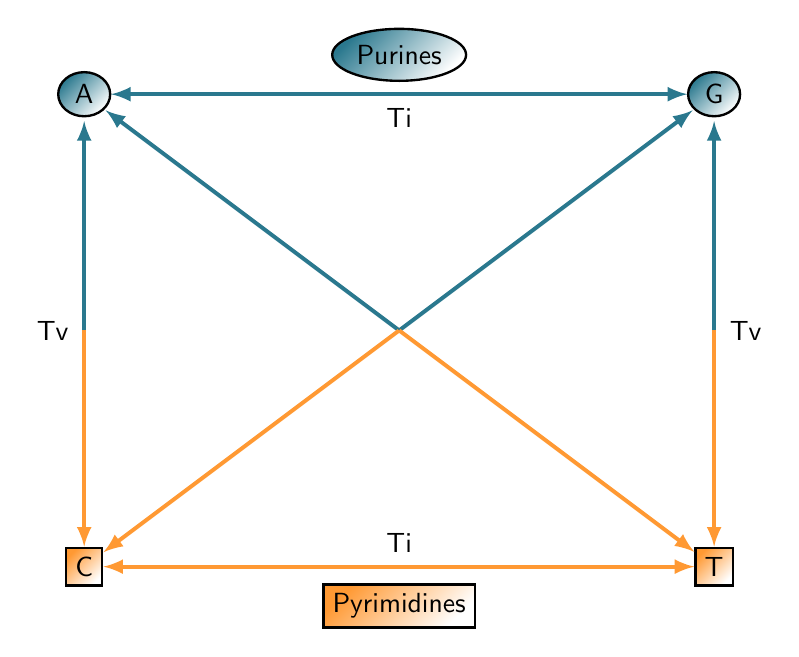
\begin{tikzpicture}
\draw [line width=0.3mm,fill=p5,left color=p5,right color=white,shading angle =45] (4,0.5) ellipse (0.85cm and 0.33cm);
\node [rectangle] at (4,0.5) (Purines) {Purines};

\draw [line width=0.3mm,fill=p5,left color=p5,right color=white,shading angle=45] (0,0) ellipse (0.33cm and 0.28cm);
\node [circle] at (0,0) (A) {A};

\draw [line width=0.3mm,fill=p5,left color=p5,right color=white,shading angle=45] (8,0) ellipse (0.33cm and 0.28cm);
\node [circle] at (8,0) (G) {G};

\node [rectangle,draw,line width=0.3mm,fill=orange!80,left color=orange!80,right color=white,shading angle=45] at (0,-6) (C) {C};

\node [rectangle,draw,line width=0.3mm,fill=orange!80,left color=orange!80,right color=white,shading angle=45] at (8,-6) (T) {T};

\node [rectangle,line width=0.3mm,draw,fill=orange!80,left color=orange!80,right color=white,shading angle=45] at (4,-6.5) (Pyrimidines) {Pyrimidines};

\draw [latex-latex,very thick,line width=0.5mm,color=p5] (A) -- (G);
\node [rectangle] at (4,-0.3) (Ti) {Ti};

\draw [latex-latex,line width=0.5mm,color=orange!80] (C) -- (T);
\node [rectangle] at (4,-5.7) (Ti) {Ti};

%\draw [latex-latex,line width=0.5mm,color=BrickRed] (A) -- (T);
%\draw [-latex,line width=0.5mm,color=p9] (4,-3) -- (T);
\draw [-latex,line width=0.5mm,color=p5] (4,-3) -- (A);

%\draw [latex-latex,line width=0.5mm,color=BrickRed] (C) -- (G);
\draw [-latex,line width=0.5mm,color=orange!80] (4,-3) -- (C);
\draw [-latex,line width=0.5mm,color=p5] (4,-3) -- (G);

%\draw [latex-latex,line width=0.5mm,color=BrickRed] (A) -- (C);
\draw [-latex,line width=0.5mm,color=p5] (0,-3) -- (A);
\draw [-latex,line width=0.5mm,color=orange!80] (0,-3) -- (C);
\node [rectangle] at (-0.4,-3) (Tv) {Tv};

%\draw [latex-latex,line width=0.5mm,color=BrickRed] (G) -- (T);
\draw [-latex,line width=0.5mm,color=p5] (8,-3) -- (G);
\draw [-latex,line width=0.5mm,color=orange!80] (8,-3) -- (T);

\draw [-latex,line width=0.5mm,color=orange!80] (4,-3) -- (T);
\node [rectangle] at (8.4,-3) (Tv) {Tv};

%\node[semi,shape border rotate=0,xscale=0.1,yscale=0.1,fill=p5,draw=p5] at (4,-2.965) {};
%\node[semi,shape border rotate=180,xscale=0.1,yscale=0.1,fill=orange!80,draw=orange!80] at (4,-3.035) {};

\end{tikzpicture}

\end{document}
